\section{Experiments}
\label{sec:experiments}

In order to evaluate the MF model, we perform several experiments using three different datasets. We start by experimenting on the normalization parameters in order to study their impact on the effectiveness of the approach. We then compare the MF ranking functions against other traditional ones. We finally discuss the consequence of \textbf{not} considering the attribute label as a source of potential relevant terms and demonstrate the effectiveness of the proposed weights.

While there are other ways to perform entity ranking on the Web of Data, e.g., one can look at the other SemSearch 2011\footnote{SemSearch2011: \url{http://km.aifb.kit.edu/ws/semsearch11}} candidates. In this evaluation we concentrate on demonstrating how the MF model specifically extends and improves the very popular PRF and DFR frameworks.

\subsection{Datasets}
\label{sec:datasets}

The datasets we are using in our experiments are the following:
\begin{description}
  \item[INEX09] a dataset of 2,491,134 triples from DBpedia containing the description of entities in English, and converted for the INEX evaluation framework~\cite{Perez-Aguera:2010:UBS};
  \item[SS10] the ``Billion Triple Challenge''\footnote{Billion Triple Challenge: \url{http://vmlion25.deri.ie}} (BTC) dataset, containing more than one billion triples, with the assessments of the SemSearch2010\footnote{SemSearch2010: \url{http://km.aifb.kit.edu/ws/semsearch10}} challenge;
  \item[SS11] the BTC dataset with the assessments of the ``Entity Search track'' of the SemSearch2011 challenge.
\end{description}
The INEX09 dataset is significantly different than the other two based on BTC. Indeed, BTC is a heterogeneous dataset, created from web crawls of several search engines. INEX09 is a highly curated dataset from DBpedia.

\subsection{Effectiveness of the MF Ranking Model}
\label{sec:mv-fields-effectiveness}

In this section, we study the impact on the retrieval performance of the normalization parameters. Next we perform a comparison between the MF extensions, i.e., BM25MF and PL2MF, against other ranking approaches. 

\subsubsection{\emph{The Normalization Parameters}}
\label{sec:norm-exp}

The effectiveness of the methods from the PRF and DFR frameworks depends on finding the right values for the normalization parameters. However, these parameters are highly dependent on the dataset.
In addition to the length normalization of field-based ranking function, the MF ranking model offers an additional normalization on the attribute's cardinality.

The Figures~\ref{fig:bm25mf-norm} and~\ref{fig:pl2mf-norm} depict the impact of the normalization parameters on the retrieval performance of BM25MF and PL2MF respectively. Each figure depicts the Mean Average Precision (MAP) scores on the three datasets for BM25MF (resp., PL2MF), with the value normalization parameter $b_v$ (resp., $c_v$) on the $x$ axis and the MAP score on the $y$ axis. Each curve plots the results with a fixed attribute normalization parameter $b_a$ (resp., $c_a$). The grid of parameters values in Figure~\ref{fig:bm25mf-norm} ranges from $0$ to $1$ with a step of $0.1$. In Figure~\ref{fig:pl2mf-norm}, the grid ranges from $0.5$ to $10.5$ with a step of $1$. Although these parameters can be attribute and value-specific, this experiment considers a constant parameter in order to reduce the number of combinations and to lower the variability of the results. Dashed lines depict the MAP scores of BM25F and PL2F and solid lines the scores of their MF extension, BM25MF and PL2MF respectively.

These plots show that using a normalization on the value node provides improved performance. Indeed, the attribute normalization parameters $b_a$ and $c_a$ alone do not grasp the heterogeneity in the data, which results in lower performance when compared to the MF extensions. This indicates that the distinction of an attribute being a set of values has a positive effect on the ranking.

\begin{subfigure}[b]{.3\textwidth}
	\renewcommand\thesubfigure{\alph{subfigure}1}
	\centering
	\resizebox{\textwidth}{!}{
	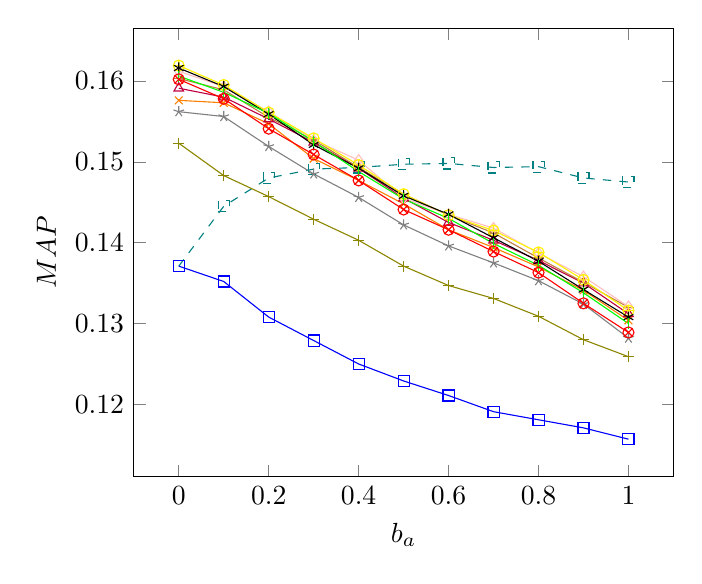
\begin{tikzpicture}
	\begin{axis}[
	xlabel=$b_a$,
	ylabel=$MAP$,
	% y label style={rotate=-90}
	]

%%%%%%%%%%%
%% x = b_v, y = b_a
%%%%%%%%%%%
%\addplot[mark=square, style=solid, color=blue] coordinates
%{ (0.0,  0.1371 ) (0.1,  0.1523 ) (0.2,  0.1562 ) (0.3,  0.1576 ) (0.4,  0.1591 ) (0.5,  0.1603 ) (0.6,  0.1612 ) (0.7,  0.1619 ) (0.8,  0.1616 ) (0.9,  0.1606 ) (1.0,  0.1602 ) };

%\addplot[mark=+, style=solid, color=olive] coordinates
%{ (0.0,  0.1352 ) (0.1,  0.1483 ) (0.2,  0.1556 ) (0.3,  0.1573 ) (0.4,  0.158 ) (0.5,  0.1589 ) (0.6,  0.1593 ) (0.7,  0.1595 ) (0.8,  0.1593 ) (0.9,  0.1586 ) (1.0,  0.1578 ) };

%\addplot[mark=star, style=solid, color=gray] coordinates
%{ (0.0,  0.1308 ) (0.1,  0.1457 ) (0.2,  0.1519 ) (0.3,  0.1547 ) (0.4,  0.1553 ) (0.5,  0.1555 ) (0.6,  0.1562 ) (0.7,  0.1561 ) (0.8,  0.1559 ) (0.9,  0.156 ) (1.0,  0.1541 ) };

%\addplot[mark=x, style=solid, color=orange] coordinates
%{ (0.0,  0.1279 ) (0.1,  0.1429 ) (0.2,  0.1485 ) (0.3,  0.1504 ) (0.4,  0.1524 ) (0.5,  0.1527 ) (0.6,  0.1527 ) (0.7,  0.1529 ) (0.8,  0.1521 ) (0.9,  0.1525 ) (1.0,  0.1509 ) };

%\addplot[mark=triangle, style=solid, color=purple] coordinates
%{ (0.0,  0.125 ) (0.1,  0.1403 ) (0.2,  0.1456 ) (0.3,  0.1477 ) (0.4,  0.1492 ) (0.5,  0.1493 ) (0.6,  0.1502 ) (0.7,  0.1496 ) (0.8,  0.1492 ) (0.9,  0.1488 ) (1.0,  0.1477 ) };

%\addplot[mark=-, style=solid, color=brown] coordinates
%{ (0.0,  0.1229 ) (0.1,  0.1371 ) (0.2,  0.1422 ) (0.3,  0.1448 ) (0.4,  0.1455 ) (0.5,  0.146 ) (0.6,  0.1455 ) (0.7,  0.146 ) (0.8,  0.1458 ) (0.9,  0.1454 ) (1.0,  0.1441 ) };

%\addplot[mark=diamond, style=solid, color=pink] coordinates
%{ (0.0,  0.1211 ) (0.1,  0.1347 ) (0.2,  0.1396 ) (0.3,  0.1416 ) (0.4,  0.1425 ) (0.5,  0.1434 ) (0.6,  0.1435 ) (0.7,  0.1434 ) (0.8,  0.1435 ) (0.9,  0.143 ) (1.0,  0.1416 ) };

%\addplot[mark=oplus, style=solid, color=yellow] coordinates
%{ (0.0,  0.1191 ) (0.1,  0.1331 ) (0.2,  0.1375 ) (0.3,  0.1394 ) (0.4,  0.1403 ) (0.5,  0.1412 ) (0.6,  0.1418 ) (0.7,  0.1415 ) (0.8,  0.1406 ) (0.9,  0.1399 ) (1.0,  0.1389 ) };

%\addplot[mark=asterisk, style=solid, color=black] coordinates
%{ (0.0,  0.1181 ) (0.1,  0.1309 ) (0.2,  0.1353 ) (0.3,  0.137 ) (0.4,  0.1378 ) (0.5,  0.1381 ) (0.6,  0.1387 ) (0.7,  0.1388 ) (0.8,  0.1377 ) (0.9,  0.1372 ) (1.0,  0.1363 ) };

%\addplot[mark=|, style=solid, color=green] coordinates
%{ (0.0,  0.1171 ) (0.1,  0.128 ) (0.2,  0.1324 ) (0.3,  0.1341 ) (0.4,  0.135 ) (0.5,  0.1351 ) (0.6,  0.1358 ) (0.7,  0.1354 ) (0.8,  0.1342 ) (0.9,  0.1338 ) (1.0,  0.1325 ) };

%\addplot[mark=otimes, style=solid, color=red] coordinates
%{ (0.0,  0.1157 ) (0.1,  0.1259 ) (0.2,  0.1282 ) (0.3,  0.1304 ) (0.4,  0.1312 ) (0.5,  0.132 ) (0.6,  0.1321 ) (0.7,  0.1316 ) (0.8,  0.1308 ) (0.9,  0.13 ) (1.0,  0.1289 ) };

%%%%%%%%%%%
%% x = b_v, y = b_a
%%%%%%%%%%%
\addplot[mark=square, style=dashed, color=teal] coordinates
{ (0, 0.1371) (.1, 0.1445) (.2, 0.148) (.3, 0.1491) (.4, 0.1493) (.5, 0.1497) (.6, 0.1498) (.7, 0.1493) (.8, 0.1494) (.9, 0.148) (1.0, 0.1475) };

\addplot[mark=square, style=solid, color=blue] coordinates
{ (0.0, 0.1371) (0.1, 0.1352) (0.2, 0.1308) (0.3, 0.1279) (0.4, 0.125) (0.5, 0.1229) (0.6, 0.1211) (0.7, 0.1191) (0.8, 0.1181) (0.9, 0.1171) (1.0, 0.1157) };

\addplot[mark=+, style=solid, color=olive] coordinates
{ (0.0, 0.1523) (0.1, 0.1483) (0.2, 0.1457) (0.3, 0.1429) (0.4, 0.1403) (0.5, 0.1371) (0.6, 0.1347) (0.7, 0.1331) (0.8, 0.1309) (0.9, 0.128) (1.0, 0.1259) };

\addplot[mark=star, style=solid, color=gray] coordinates
{ (0.0, 0.1562) (0.1, 0.1556) (0.2, 0.1519) (0.3, 0.1485) (0.4, 0.1456) (0.5, 0.1422) (0.6, 0.1396) (0.7, 0.1375) (0.8, 0.1353) (0.9, 0.1324) (1.0, 0.1282) };

\addplot[mark=x, style=solid, color=orange] coordinates
{ (0.0, 0.1576) (0.1, 0.1573) (0.2, 0.1547) (0.3, 0.1504) (0.4, 0.1477) (0.5, 0.1448) (0.6, 0.1416) (0.7, 0.1394) (0.8, 0.137) (0.9, 0.1341) (1.0, 0.1304) };

\addplot[mark=triangle, style=solid, color=purple] coordinates
{ (0.0, 0.1591) (0.1, 0.158) (0.2, 0.1553) (0.3, 0.1524) (0.4, 0.1492) (0.5, 0.1455) (0.6, 0.1425) (0.7, 0.1403) (0.8, 0.1378) (0.9, 0.135) (1.0, 0.1312) };

\addplot[mark=-, style=solid, color=brown] coordinates
{ (0.0, 0.1603) (0.1, 0.1589) (0.2, 0.1555) (0.3, 0.1527) (0.4, 0.1493) (0.5, 0.146) (0.6, 0.1434) (0.7, 0.1412) (0.8, 0.1381) (0.9, 0.1351) (1.0, 0.132) };

\addplot[mark=diamond, style=solid, color=pink] coordinates
{ (0.0, 0.1612) (0.1, 0.1593) (0.2, 0.1562) (0.3, 0.1527) (0.4, 0.1502) (0.5, 0.1455) (0.6, 0.1435) (0.7, 0.1418) (0.8, 0.1387) (0.9, 0.1358) (1.0, 0.1321) };

\addplot[mark=oplus, style=solid, color=yellow] coordinates
{ (0.0, 0.1619) (0.1, 0.1595) (0.2, 0.1561) (0.3, 0.1529) (0.4, 0.1496) (0.5, 0.146) (0.6, 0.1434) (0.7, 0.1415) (0.8, 0.1388) (0.9, 0.1354) (1.0, 0.1316) };

\addplot[mark=asterisk, style=solid, color=black] coordinates
{ (0.0, 0.1616) (0.1, 0.1593) (0.2, 0.1559) (0.3, 0.1521) (0.4, 0.1492) (0.5, 0.1458) (0.6, 0.1435) (0.7, 0.1406) (0.8, 0.1377) (0.9, 0.1342) (1.0, 0.1308) };

\addplot[mark=|, style=solid, color=green] coordinates
{ (0.0, 0.1606) (0.1, 0.1586) (0.2, 0.156) (0.3, 0.1525) (0.4, 0.1488) (0.5, 0.1454) (0.6, 0.143) (0.7, 0.1399) (0.8, 0.1372) (0.9, 0.1338) (1.0, 0.13) };

\addplot[mark=otimes, style=solid, color=red] coordinates
{ (0.0, 0.1602) (0.1, 0.1578) (0.2, 0.1541) (0.3, 0.1509) (0.4, 0.1477) (0.5, 0.1441) (0.6, 0.1416) (0.7, 0.1389) (0.8, 0.1363) (0.9, 0.1325) (1.0, 0.1289) };

\end{axis}
\end{tikzpicture}}

	\caption{INEX09}
\end{subfigure}
\quad%
\begin{subfigure}[b]{.3\textwidth}
	\addtocounter{subfigure}{-1}
	\renewcommand\thesubfigure{\alph{subfigure}2}
	\centering
	\resizebox{\textwidth}{!}{
	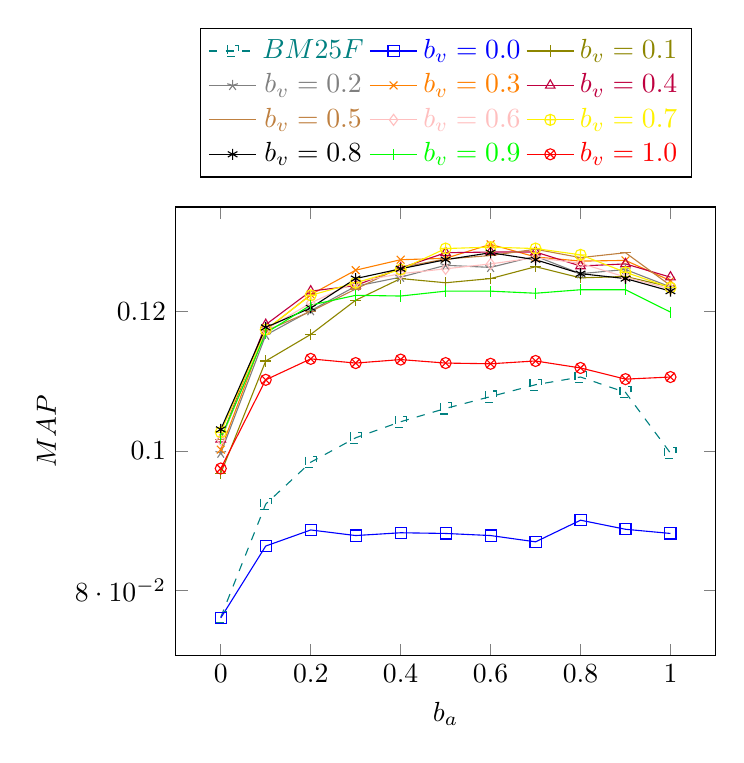
\begin{tikzpicture}
	\begin{axis}[
	  legend entries={
	    [teal]$BM25F$,
		[blue]$b_v = 0.0$,
	 	[olive]$b_v = 0.1$,
	  	[gray]$b_v = 0.2$,
	  	[orange]$b_v = 0.3$,
		[purple]$b_v = 0.4$,
	 	[brown]$b_v = 0.5$,
	  	[pink]$b_v = 0.6$,
	  	[yellow]$b_v = 0.7$,
		[black]$b_v = 0.8$,
	 	[green]$b_v = 0.9$,
	 	[red]$b_v = 1.0$
	  },
	  legend columns=3,
      legend style={at={(0.5,1.4)},anchor=north},
	  xlabel=$b_a$,
	  ylabel=$MAP$,
	  % y label style={rotate=-90},
	]

%%%%%%%%%%%
%% x = c_v, y = c_a
%%%%%%%%%%%
%\addplot[mark=square, style=solid, color=blue] coordinates
%{ (0.0, 0.0761) (0.1, 0.0968) (0.2, 0.0997) (0.3, 0.1002) (0.4, 0.1017) (0.5, 0.1016) (0.6, 0.1016) (0.7, 0.1027) (0.8, 0.1031) (0.9, 0.1018) (1.0, 0.0975) };

%\addplot[mark=+, style=solid, color=olive] coordinates
%{ (0.0, 0.0864) (0.1, 0.1129) (0.2, 0.1166) (0.3, 0.1173) (0.4, 0.1181) (0.5, 0.1172) (0.6, 0.1174) (0.7, 0.1174) (0.8, 0.1177) (0.9, 0.1169) (1.0, 0.1102) };

%\addplot[mark=star, style=solid, color=gray] coordinates
%{ (0.0, 0.0887) (0.1, 0.1167) (0.2, 0.1201) (0.3, 0.1224) (0.4, 0.1229) (0.5, 0.12) (0.6, 0.1212) (0.7, 0.1223) (0.8, 0.1205) (0.9, 0.1209) (1.0, 0.1132) };

%\addplot[mark=x, style=solid, color=orange] coordinates
%{ (0.0, 0.0879) (0.1, 0.1216) (0.2, 0.1236) (0.3, 0.1259) (0.4, 0.1237) (0.5, 0.1232) (0.6, 0.1242) (0.7, 0.1241) (0.8, 0.1247) (0.9, 0.1223) (1.0, 0.1126) };

%\addplot[mark=triangle, style=solid, color=purple] coordinates
%{ (0.0, 0.0883) (0.1, 0.1247) (0.2, 0.1249) (0.3, 0.1274) (0.4, 0.1262) (0.5, 0.1263) (0.6, 0.1254) (0.7, 0.126) (0.8, 0.1261) (0.9, 0.1222) (1.0, 0.1131) };

%\addplot[mark=-, style=solid, color=brown] coordinates
%{ (0.0, 0.0882) (0.1, 0.1241) (0.2, 0.1266) (0.3, 0.1276) (0.4, 0.1284) (0.5, 0.1275) (0.6, 0.1261) (0.7, 0.129) (0.8, 0.1274) (0.9, 0.1229) (1.0, 0.1126) };

%\addplot[mark=diamond, style=solid, color=pink] coordinates
%{ (0.0, 0.0879) (0.1, 0.1247) (0.2, 0.1263) (0.3, 0.1296) (0.4, 0.1285) (0.5, 0.128) (0.6, 0.1268) (0.7, 0.1292) (0.8, 0.1284) (0.9, 0.1229) (1.0, 0.1125) };

%\addplot[mark=oplus, style=solid, color=yellow] coordinates
%{ (0.0, 0.087) (0.1, 0.1264) (0.2, 0.1279) (0.3, 0.1278) (0.4, 0.1285) (0.5, 0.1289) (0.6, 0.1277) (0.7, 0.129) (0.8, 0.1274) (0.9, 0.1226) (1.0, 0.1129) };

%\addplot[mark=asterisk, style=solid, color=black] coordinates
%{ (0.0, 0.0901) (0.1, 0.1248) (0.2, 0.1254) (0.3, 0.1272) (0.4, 0.1265) (0.5, 0.1277) (0.6, 0.1269) (0.7, 0.1281) (0.8, 0.1254) (0.9, 0.1231) (1.0, 0.1119) };

%\addplot[mark=|, style=solid, color=green] coordinates
%{ (0.0, 0.0888) (0.1, 0.125) (0.2, 0.126) (0.3, 0.1273) (0.4, 0.1268) (0.5, 0.1284) (0.6, 0.1249) (0.7, 0.1256) (0.8, 0.1247) (0.9, 0.1231) (1.0, 0.1103) };

%\addplot[mark=otimes, style=solid, color=red] coordinates
%{ (0.0, 0.0882) (0.1, 0.1235) (0.2, 0.1235) (0.3, 0.1244) (0.4, 0.1249) (0.5, 0.1237) (0.6, 0.1232) (0.7, 0.1234) (0.8, 0.1229) (0.9, 0.1199) (1.0, 0.1106) };

%%%%%%%%%%%
%% x = b_a, y = b_v
%%%%%%%%%%%
\addplot[mark=square, style=dashed, color=teal] coordinates
{ (0, 0.0762) (.1, 0.0924) (.2, 0.0984) (.3, 0.1019) (.4, 0.1042) (.5, 0.1061) (.6, 0.1078) (.7, 0.1095) (.8, 0.1106) (.9, 0.1084) (1.0, 0.0997) };

\addplot[mark=square, style=solid, color=blue] coordinates
{ (0.0, 0.0761) (0.1, 0.0864) (0.2, 0.0887) (0.3, 0.0879) (0.4, 0.0883) (0.5, 0.0882) (0.6, 0.0879) (0.7, 0.087) (0.8, 0.0901) (0.9, 0.0888) (1.0, 0.0882) };

\addplot[mark=+, style=solid, color=olive] coordinates
{ (0.0, 0.0968) (0.1, 0.1129) (0.2, 0.1167) (0.3, 0.1216) (0.4, 0.1247) (0.5, 0.1241) (0.6, 0.1247) (0.7, 0.1264) (0.8, 0.1248) (0.9, 0.125) (1.0, 0.1235) };

\addplot[mark=star, style=solid, color=gray] coordinates
{ (0.0, 0.0997) (0.1, 0.1166) (0.2, 0.1201) (0.3, 0.1236) (0.4, 0.1249) (0.5, 0.1266) (0.6, 0.1263) (0.7, 0.1279) (0.8, 0.1254) (0.9, 0.126) (1.0, 0.1235) };

\addplot[mark=x, style=solid, color=orange] coordinates
{ (0.0, 0.1002) (0.1, 0.1173) (0.2, 0.1224) (0.3, 0.1259) (0.4, 0.1274) (0.5, 0.1276) (0.6, 0.1296) (0.7, 0.1278) (0.8, 0.1272) (0.9, 0.1273) (1.0, 0.1244) };

\addplot[mark=triangle, style=solid, color=purple] coordinates
{ (0.0, 0.1017) (0.1, 0.1181) (0.2, 0.1229) (0.3, 0.1237) (0.4, 0.1262) (0.5, 0.1284) (0.6, 0.1285) (0.7, 0.1285) (0.8, 0.1265) (0.9, 0.1268) (1.0, 0.1249) };

\addplot[mark=-, style=solid, color=brown] coordinates
{ (0.0, 0.1016) (0.1, 0.1172) (0.2, 0.12) (0.3, 0.1232) (0.4, 0.1263) (0.5, 0.1275) (0.6, 0.128) (0.7, 0.1289) (0.8, 0.1277) (0.9, 0.1284) (1.0, 0.1237) };

\addplot[mark=diamond, style=solid, color=pink] coordinates
{ (0.0, 0.1016) (0.1, 0.1174) (0.2, 0.1212) (0.3, 0.1242) (0.4, 0.1254) (0.5, 0.1261) (0.6, 0.1268) (0.7, 0.1277) (0.8, 0.1269) (0.9, 0.1249) (1.0, 0.1232) };

\addplot[mark=oplus, style=solid, color=yellow] coordinates
{ (0.0, 0.1027) (0.1, 0.1174) (0.2, 0.1223) (0.3, 0.1241) (0.4, 0.126) (0.5, 0.129) (0.6, 0.1292) (0.7, 0.129) (0.8, 0.1281) (0.9, 0.1256) (1.0, 0.1234) };

\addplot[mark=asterisk, style=solid, color=black] coordinates
{ (0.0, 0.1031) (0.1, 0.1177) (0.2, 0.1205) (0.3, 0.1247) (0.4, 0.1261) (0.5, 0.1274) (0.6, 0.1284) (0.7, 0.1274) (0.8, 0.1254) (0.9, 0.1247) (1.0, 0.1229) };

\addplot[mark=|, style=solid, color=green] coordinates
{ (0.0, 0.1018) (0.1, 0.1169) (0.2, 0.1209) (0.3, 0.1223) (0.4, 0.1222) (0.5, 0.1229) (0.6, 0.1229) (0.7, 0.1226) (0.8, 0.1231) (0.9, 0.1231) (1.0, 0.1199) };

\addplot[mark=otimes, style=solid, color=red] coordinates
{ (0.0, 0.0975) (0.1, 0.1102) (0.2, 0.1132) (0.3, 0.1126) (0.4, 0.1131) (0.5, 0.1126) (0.6, 0.1125) (0.7, 0.1129) (0.8, 0.1119) (0.9, 0.1103) (1.0, 0.1106) };

\end{axis}
\end{tikzpicture}}

	\caption{SS10}
\end{subfigure}
\quad%
\begin{subfigure}[b]{.3\textwidth}
	\addtocounter{subfigure}{-1}
	\renewcommand\thesubfigure{\alph{subfigure}3}
	\centering
	\resizebox{\textwidth}{!}{
	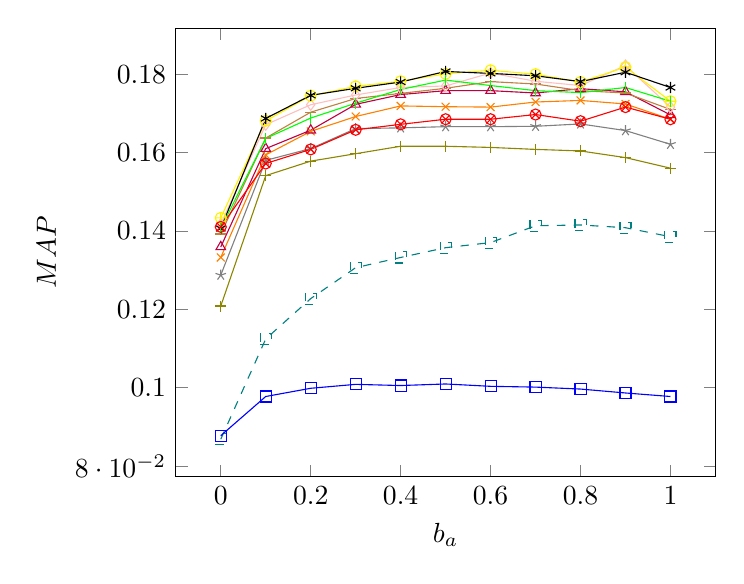
\begin{tikzpicture}
	\begin{axis}[
		xlabel=$b_a$,
		ylabel=$MAP$,
		% y label style={rotate=-90},
	]

%%%%%%%%%%%
%% x = b_v, y = b_a
%%%%%%%%%%%
%\addplot[mark=square, style=solid, color=blue] coordinates
%{ (0.0,  0.0877) (0.1,  0.1208) (0.2,  0.1287) (0.3,  0.1332) (0.4,  0.1359) (0.5,  0.1392) (0.6,  0.1417) (0.7,  0.1433) (0.8, 0.1406) (0.9, 0.1406) (1.0, 0.141) };

%\addplot[mark=+, style=solid, color=olive] coordinates
%{ (0.0,  0.0977) (0.1, 0.1541 ) (0.2,  0.158) (0.3, 0.1594) (0.4,  0.161) (0.5,  0.1637) (0.6, 0.1671) (0.7,  0.1681) (0.8, 0.1687) (0.9,  0.1636) (1.0,  0.1572) };

%\addplot[mark=star, style=solid, color=gray] coordinates
%{ (0.0, 0.0998 ) (0.1,  0.1578) (0.2,  0.161) (0.3,  0.1654) (0.4,  0.1657) (0.5, 0.1703) (0.6,  0.1722) (0.7, 0.1745) (0.8,  0.1746) (0.9,  0.1688) (1.0, 0.1608) };

%\addplot[mark=x, style=solid, color=orange] coordinates
%{ (0.0,  0.1008) (0.1,  0.1597) (0.2,  0.1661) (0.3,  0.1692) (0.4,  0.1723) (0.5, 0.1738) (0.6, 0.1747) (0.7, 0.1769) (0.8,  0.1764) (0.9,  0.1726) (1.0, 0.1658) };

%\addplot[mark=triangle, style=solid, color=purple] coordinates
%{ (0.0,  0.1005) (0.1,  0.1616) (0.2,  0.1663) (0.3,  0.1719) (0.4, 0.1748 ) (0.5, 0.1751) (0.6,0.1766 ) (0.7, 0.1782) (0.8,  0.178) (0.9,  0.1761) (1.0,  0.1672) };

%\addplot[mark=-, style=solid, color=brown] coordinates
%{ (0.0,  0.1009) (0.1,  0.1616) (0.2,  0.1666) (0.3,  0.1717) (0.4,  0.1758) (0.5, 0.1764 ) (0.6, 0.177) (0.7, 0.1801) (0.8,  0.1807) (0.9,  0.1785) (1.0, 0.1685) };

%\addplot[mark=diamond, style=solid, color=pink] coordinates
%{ (0.0,  0.1003) (0.1,  0.1613) (0.2,  0.1666) (0.3,  0.1716) (0.4,  0.1758) (0.5, 0.1781) (0.6, 0.1803) (0.7, 0.181) (0.8,  0.1802) (0.9,  0.1771) (1.0,  0.1685) };

%\addplot[mark=oplus, style=solid, color=yellow] coordinates
%{ (0.0,  0.1001) (0.1,  0.1608) (0.2,  0.1667) (0.3,  0.1729) (0.4,  0.1752) (0.5, 0.1775) (0.6, 0.1782) (0.7, 0.18) (0.8, 0.1796 ) (0.9,  0.1758) (1.0,  0.1697) };

%\addplot[mark=asterisk, style=solid, color=black] coordinates
%{ (0.0, 0.0996 ) (0.1,  0.1604) (0.2, 0.1673 ) (0.3, 0.1733 ) (0.4, 0.1763 ) (0.5, 0.1758 ) (0.6, 0.1771) (0.7, 0.178) (0.8,  0.1781) (0.9,  0.1753) (1.0,  0.168) };

%\addplot[mark=|, style=solid, color=green] coordinates
%{ (0.0,  0.0986) (0.1, 0.1587 ) (0.2, 0.1656 ) (0.3, 0.1724 ) (0.4, 0.1755 ) (0.5, 0.1752 ) (0.6, 0.1822) (0.7, 0.1818) (0.8, 0.1805 ) (0.9, 0.1766 ) (1.0, 0.1716 )
%};

%\addplot[mark=otimes, style=solid, color=red] coordinates
%{ (0.0, 0.0977 ) (0.1, 0.156 ) (0.2, 0.1621 ) (0.3, 0.1685 ) (0.4, 0.1696 ) (0.5, 0.171 ) (0.6, 0.1716 ) (0.7, 0.1731 ) (0.8, 0.1766) (0.9, 0.1731) (1.0, 0.1685 ) };

%%%%%%%%%%%
%% x = b_a, y = b_v
%%%%%%%%%%%

\addplot[mark=square, style=dashed, color=teal] coordinates
{ (0, 0.0868) (.1, 0.1124) (.2, 0.1227) (.3, 0.1306) (.4, 0.1332) (.5, 0.1357) (.6, 0.137) (.7, 0.1413) (.8, 0.1415) (.9, 0.1408) (1.0, 0.1385) };

\addplot[mark=square, style=solid, color=blue] coordinates
{ (0.0, 0.0877) (0.1, 0.0977) (0.2, 0.0998) (0.3, 0.1008) (0.4, 0.1005) (0.5, 0.1009) (0.6, 0.1003) (0.7, 0.1001) (0.8, 0.0996) (0.9, 0.0986) (1.0, 0.0977) };

\addplot[mark=+, style=solid, color=olive] coordinates
{ (0.0, 0.1208) (0.1, 0.1541) (0.2, 0.1578) (0.3, 0.1597) (0.4, 0.1616) (0.5, 0.1616) (0.6, 0.1613) (0.7, 0.1608) (0.8, 0.1604) (0.9, 0.1587) (1.0, 0.156) };

\addplot[mark=star, style=solid, color=gray] coordinates
{ (0.0, 0.1287) (0.1, 0.158) (0.2, 0.161) (0.3, 0.1661) (0.4, 0.1663) (0.5, 0.1666) (0.6, 0.1666) (0.7, 0.1667) (0.8, 0.1673) (0.9, 0.1656) (1.0, 0.1621) };

\addplot[mark=x, style=solid, color=orange] coordinates
{ (0.0, 0.1332) (0.1, 0.1594) (0.2, 0.1654) (0.3, 0.1692) (0.4, 0.1719) (0.5, 0.1717) (0.6, 0.1716) (0.7, 0.1729) (0.8, 0.1733) (0.9, 0.1724) (1.0, 0.1685) };

\addplot[mark=triangle, style=solid, color=purple] coordinates
{ (0.0, 0.1359) (0.1, 0.161) (0.2, 0.1657) (0.3, 0.1723) (0.4, 0.1748) (0.5, 0.1758) (0.6, 0.1758) (0.7, 0.1752) (0.8, 0.1763) (0.9, 0.1755) (1.0, 0.1696) };

\addplot[mark=-, style=solid, color=brown] coordinates
{ (0.0, 0.1392) (0.1, 0.1637) (0.2, 0.1703) (0.3, 0.1738) (0.4, 0.1751) (0.5, 0.1764) (0.6, 0.1781) (0.7, 0.1775) (0.8, 0.1758) (0.9, 0.1752) (1.0, 0.171) };

\addplot[mark=diamond, style=solid, color=pink] coordinates
{ (0.0, 0.1417) (0.1, 0.1671) (0.2, 0.1722) (0.3, 0.1747) (0.4, 0.1766) (0.5, 0.177) (0.6, 0.1803) (0.7, 0.1782) (0.8, 0.1771) (0.9, 0.1822) (1.0, 0.1716) };

\addplot[mark=oplus, style=solid, color=yellow] coordinates
{ (0.0, 0.1433) (0.1, 0.1681) (0.2, 0.1745) (0.3, 0.1769) (0.4, 0.1782) (0.5, 0.1801) (0.6, 0.181) (0.7, 0.18) (0.8, 0.178) (0.9, 0.1818) (1.0, 0.1731) };

\addplot[mark=asterisk, style=solid, color=black] coordinates
{ (0.0, 0.1406) (0.1, 0.1687) (0.2, 0.1746) (0.3, 0.1764) (0.4, 0.178) (0.5, 0.1807) (0.6, 0.1802) (0.7, 0.1796) (0.8, 0.1781) (0.9, 0.1805) (1.0, 0.1766) };

\addplot[mark=|, style=solid, color=green] coordinates
{ (0.0, 0.1406) (0.1, 0.1636) (0.2, 0.1688) (0.3, 0.1726) (0.4, 0.1761) (0.5, 0.1785) (0.6, 0.1771) (0.7, 0.1758) (0.8, 0.1753) (0.9, 0.1766) (1.0, 0.1731) };

\addplot[mark=otimes, style=solid, color=red] coordinates
{ (0.0, 0.141) (0.1, 0.1572) (0.2, 0.1608) (0.3, 0.1658) (0.4, 0.1672) (0.5, 0.1685) (0.6, 0.1685) (0.7, 0.1697) (0.8, 0.168) (0.9, 0.1716) (1.0, 0.1685) };

\end{axis}
\end{tikzpicture}}
\caption{SS11}
\end{subfigure}


\begin{subfigure}[b]{.3\textwidth}
	\renewcommand\thesubfigure{\alph{subfigure}1}
	\centering
	\resizebox{\textwidth}{!}{
	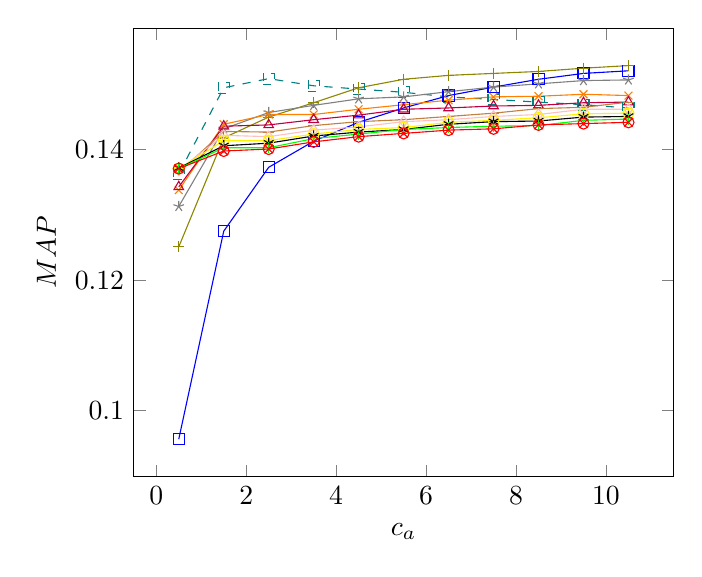
\begin{tikzpicture}
		\begin{axis}[
		xlabel=$c_a$,
		ylabel=$MAP$,
		% y label style={rotate=-90}
	]
%%%%%%%%%%%%%%%%%%%%
%%% x=cv y=ca, from 5 to 50, with step of 5
%%%%%%%%%%%%%%%%%%%%
%%\addplot[mark=square, style=solid, color=blue] coordinates

%\addplot[mark=+, style=solid, color=olive] coordinates
%{ (0, 0.1492) (5, 0.1451) (10, 0.1425) (15, 0.1411) (20, 0.1397) (25, 0.1381) (30, 0.1373) (35, 0.137) (40, 0.1365) (45, 0.136) (50, 0.1356) };

%\addplot[mark=star, style=solid, color=gray] coordinates
%{ (0, 0.1468) (5, 0.1469) (10, 0.1444) (15, 0.1421) (20, 0.1408) (25, 0.1397) (30, 0.1387) (35, 0.1381) (40, 0.1377) (45, 0.1372) (50, 0.1369) };

%\addplot[mark=x, style=solid, color=orange] coordinates
%{ (0, 0.1452) (5, 0.1476) (10, 0.1442) (15, 0.1419) (20, 0.1407) (25, 0.1397) (30, 0.1388) (35, 0.1382) (40, 0.1377) (45, 0.1373) (50, 0.1369) };

%\addplot[mark=triangle, style=solid, color=purple] coordinates
%{ (0, 0.1443) (5, 0.1475) (10, 0.1435) (15, 0.1415) (20, 0.1403) (25, 0.1393) (30, 0.1384) (35, 0.1379) (40, 0.1375) (45, 0.1371) (50, 0.1369) };

%\addplot[mark=-, style=solid, color=brown] coordinates
%{ (0, 0.1431) (5, 0.1472) (10, 0.1435) (15, 0.1413) (20, 0.1399) (25, 0.139) (30, 0.1384) (35, 0.1378) (40, 0.1374) (45, 0.1371) (50, 0.1367) };

%\addplot[mark=diamond, style=solid, color=pink] coordinates
%{ (0, 0.1422) (5, 0.1472) (10, 0.1432) (15, 0.1412) (20, 0.1401) (25, 0.1393) (30, 0.1385) (35, 0.1379) (40, 0.1376) (45, 0.1372) (50, 0.137) };

%\addplot[mark=oplus, style=solid, color=yellow] coordinates
%{ (0, 0.1418) (5, 0.1473) (10, 0.1431) (15, 0.1411) (20, 0.1401) (25, 0.1392) (30, 0.1387) (35, 0.1383) (40, 0.1378) (45, 0.1374) (50, 0.137) };

%\addplot[mark=asterisk, style=solid, color=black] coordinates
%{ (0, 0.141) (5, 0.147) (10, 0.1431) (15, 0.1411) (20, 0.1402) (25, 0.1392) (30, 0.1389) (35, 0.1383) (40, 0.1378) (45, 0.1373) (50, 0.137) };

%\addplot[mark=|, style=solid, color=green] coordinates
%{ (0, 0.1406) (5, 0.1468) (10, 0.143) (15, 0.1413) (20, 0.1403) (25, 0.1394) (30, 0.1387) (35, 0.1382) (40, 0.1377) (45, 0.1372) (50, 0.1369) };

%\addplot[mark=otimes, style=solid, color=red] coordinates
%{ (0, 0.1403) (5, 0.1466) (10, 0.1431) (15, 0.1412) (20, 0.1402) (25, 0.1394) (30, 0.1386) (35, 0.1383) (40, 0.1379) (45, 0.1373) (50, 0.1368) };

%%%%%%%%%%%%%%%%%%%%
%%% x=ca y=cv, from 0.5 to 10.5, with step of 1
%%%%%%%%%%%%%%%%%%%%
\addplot[mark=square, style=dashed, color=teal] coordinates
{ (0.5, 0.1363) (1.5, 0.1495) (2.5, 0.1509) (3.5, 0.1498) (4.5, 0.1493) (5.5, 0.1488) (6.5, 0.1481) (7.5, 0.1477) (8.5, 0.1473) (9.5, 0.1469) (10.5, 0.1464) };

\addplot[mark=square, style=solid, color=blue] coordinates
{ (0.5, 0.0956) (1.5, 0.1275) (2.5, 0.1373) (3.5, 0.1413) (4.5, 0.1442) (5.5, 0.1464) (6.5, 0.1483) (7.5, 0.1496) (8.5, 0.1508) (9.5, 0.1517) (10.5, 0.1521) };

\addplot[mark=+, style=solid, color=olive] coordinates
{ (0.5, 0.1251) (1.5, 0.1418) (2.5, 0.145) (3.5, 0.1472) (4.5, 0.1495) (5.5, 0.1508) (6.5, 0.1514) (7.5, 0.1517) (8.5, 0.152) (9.5, 0.1525) (10.5, 0.1529) };

\addplot[mark=star, style=solid, color=gray] coordinates
{ (0.5, 0.1313) (1.5, 0.1432) (2.5, 0.1457) (3.5, 0.1468) (4.5, 0.1478) (5.5, 0.1481) (6.5, 0.1489) (7.5, 0.1496) (8.5, 0.1501) (9.5, 0.1506) (10.5, 0.1507) };

\addplot[mark=x, style=solid, color=orange] coordinates
{ (0.5, 0.1338) (1.5, 0.1439) (2.5, 0.1454) (3.5, 0.1454) (4.5, 0.1462) (5.5, 0.1469) (6.5, 0.1476) (7.5, 0.1481) (8.5, 0.1482) (9.5, 0.1485) (10.5, 0.1483) };

\addplot[mark=triangle, style=solid, color=purple] coordinates
{ (0.5, 0.1343) (1.5, 0.1436) (2.5, 0.1438) (3.5, 0.1446) (4.5, 0.1453) (5.5, 0.1462) (6.5, 0.1464) (7.5, 0.1467) (8.5, 0.1468) (9.5, 0.1472) (10.5, 0.1473) };

\addplot[mark=-, style=solid, color=brown] coordinates
{ (0.5, 0.1365) (1.5, 0.1428) (2.5, 0.1427) (3.5, 0.1437) (4.5, 0.1443) (5.5, 0.1446) (6.5, 0.1451) (7.5, 0.1456) (8.5, 0.1463) (9.5, 0.1465) (10.5, 0.1473) };

\addplot[mark=diamond, style=solid, color=pink] coordinates
{ (0.5, 0.1369) (1.5, 0.1422) (2.5, 0.142) (3.5, 0.143) (4.5, 0.1435) (5.5, 0.1443) (6.5, 0.1446) (7.5, 0.1451) (8.5, 0.1454) (9.5, 0.1462) (10.5, 0.1462) };

\addplot[mark=oplus, style=solid, color=yellow] coordinates
{ (0.5, 0.1371) (1.5, 0.1414) (2.5, 0.1414) (3.5, 0.1424) (4.5, 0.1431) (5.5, 0.1434) (6.5, 0.1442) (7.5, 0.1445) (8.5, 0.1449) (9.5, 0.1455) (10.5, 0.1456) };

\addplot[mark=asterisk, style=solid, color=black] coordinates
{ (0.5, 0.1372) (1.5, 0.1406) (2.5, 0.141) (3.5, 0.1421) (4.5, 0.1427) (5.5, 0.1431) (6.5, 0.1439) (7.5, 0.1443) (8.5, 0.1444) (9.5, 0.145) (10.5, 0.1451) };

\addplot[mark=|, style=solid, color=green] coordinates
{ (0.5, 0.1371) (1.5, 0.1403) (2.5, 0.1403) (3.5, 0.1417) (4.5, 0.1424) (5.5, 0.1431) (6.5, 0.1434) (7.5, 0.1436) (8.5, 0.1437) (9.5, 0.1445) (10.5, 0.1447) };

\addplot[mark=otimes, style=solid, color=red] coordinates
{ (0.5, 0.1371) (1.5, 0.1398) (2.5, 0.1401) (3.5, 0.1412) (4.5, 0.142) (5.5, 0.1425) (6.5, 0.143) (7.5, 0.1432) (8.5, 0.1438) (9.5, 0.144) (10.5, 0.1442) };

\end{axis}
\end{tikzpicture}}

	\caption{INEX09}
\end{subfigure}
\quad%
\begin{subfigure}[b]{.3\textwidth}
	\addtocounter{subfigure}{-1}
	\renewcommand\thesubfigure{\alph{subfigure}2}
	\centering
	\resizebox{\textwidth}{!}{
	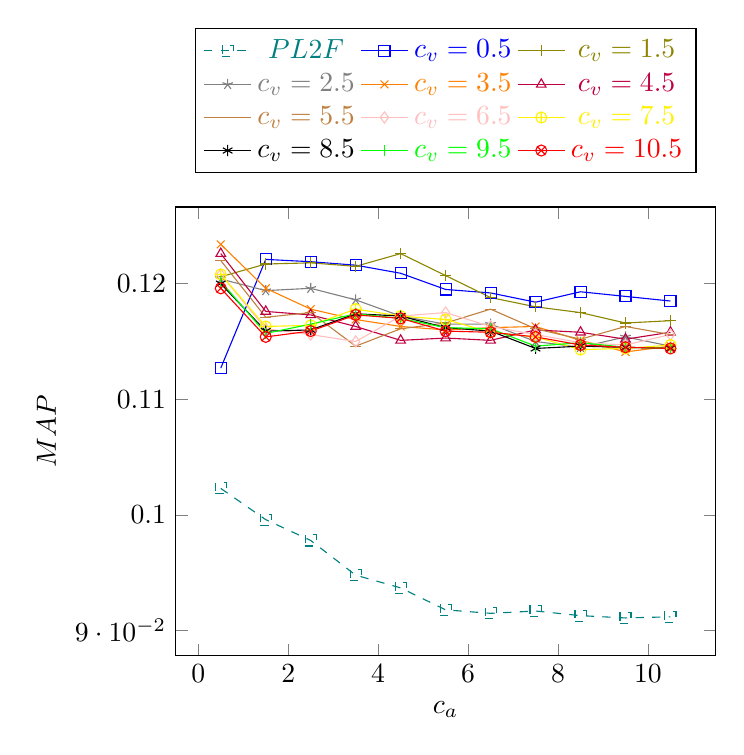
\begin{tikzpicture}
	\begin{axis}[
	  legend entries={
	    [teal]$PL2F$,
		[blue]$c_v = 0.5$,
	 	[olive]$c_v = 1.5$,
	  	[gray]$c_v = 2.5$,
	  	[orange]$c_v = 3.5$,
		[purple]$c_v = 4.5$,
	 	[brown]$c_v = 5.5$,
	  	[pink]$c_v = 6.5$,
	  	[yellow]$c_v = 7.5$,
		[black]$c_v = 8.5$,
	 	[green]$c_v = 9.5$,
	 	[red]$c_v = 10.5$
	  },
	  legend columns=3,
	legend style={at={(0.5,1.4)},anchor=north},
	 xlabel=$c_a$,
	ylabel=$MAP$,
	% y label style={rotate=-90},
	]

%%%%%%%%%%%%%%%%%%%%
%%% x=cv y=ca, from 5 to 50, with step of 5
%%%%%%%%%%%%%%%%%%%%
%\addplot[mark=square, style=solid, color=blue] coordinates
%{ (5, ) (10, ) (15, ) (20, ) (25, ) (30, ) (35, ) (40, ) (45, ) (50, )  };

%\addplot[mark=+, style=solid, color=olive] coordinates
%{ (0, 0.0928) (5, 0.1153) (10, 0.1174) (15, 0.116) (20, 0.1167) (25, 0.115) (30, 0.1136) (35, 0.1137) (40, 0.1139) (45, 0.1132) (50, 0.1136)  };

%\addplot[mark=star, style=solid, color=gray] coordinates
%{ (0, 0.0913) (5, 0.1158) (10, 0.1144) (15, 0.113) (20, 0.1136) (25, 0.114) (30, 0.1126) (35, 0.1127) (40, 0.112) (45, 0.1114) (50, 0.1106)  };

%\addplot[mark=x, style=solid, color=orange] coordinates
%{ (0, 0.0886) (5, 0.115) (10, 0.114) (15, 0.1127) (20, 0.1123) (25, 0.1123) (30, 0.1122) (35, 0.1121) (40, 0.1113) (45, 0.1105) (50, 0.1104)  };

%\addplot[mark=triangle, style=solid, color=purple] coordinates
%{ (0, 0.0879) (5, 0.114) (10, 0.1132) (15, 0.112) (20, 0.1124) (25, 0.1119) (30, 0.111) (35, 0.1111) (40, 0.1097) (45, 0.1097) (50, 0.1098)  };

%\addplot[mark=-, style=solid, color=brown] coordinates
%{ (0, 0.0868) (5, 0.1137) (10, 0.1137) (15, 0.1125) (20, 0.1111) (25, 0.1105) (30, 0.1101) (35, 0.11) (40, 0.1099) (45, 0.109) (50, 0.1091)  };

%\addplot[mark=diamond, style=solid, color=pink] coordinates
%{ (0, 0.0864) (5, 0.1131) (10, 0.1126) (15, 0.111) (20, 0.1104) (25, 0.1092) (30, 0.1092) (35, 0.1093) (40, 0.109) (45, 0.1081) (50, 0.1082)  };

%\addplot[mark=oplus, style=solid, color=yellow] coordinates
%{ (0, 0.0856) (5, 0.1129) (10, 0.1109) (15, 0.1105) (20, 0.1097) (25, 0.1084) (30, 0.1082) (35, 0.1076) (40, 0.1081) (45, 0.1079) (50, 0.107)  };

%\addplot[mark=asterisk, style=solid, color=black] coordinates
%{ (0, 0.0845) (5, 0.1124) (10, 0.1115) (15, 0.1102) (20, 0.1095) (25, 0.1083) (30, 0.1079) (35, 0.1078) (40, 0.1075) (45, 0.1073) (50, 0.1066)  };

%\addplot[mark=|, style=solid, color=green] coordinates
%{ (0, 0.0833) (5, 0.1121) (10, 0.1113) (15, 0.1099) (20, 0.1095) (25, 0.1087) (30, 0.1081) (35, 0.1081) (40, 0.1077) (45, 0.1068) (50, 0.1059)  };

%\addplot[mark=otimes, style=solid, color=red] coordinates
%{ (0, 0.0824) (5, 0.1116) (10, 0.1109) (15, 0.1099) (20, 0.1095) (25, 0.1086) (30, 0.1077) (35, 0.1077) (40, 0.1076) (45, 0.107) (50, 0.1068)  };

%%%%%%%%%%%%%%%%%%%%
%%% x=ca y=cv, from 0.5 to 10.5, with step of 1
%%%%%%%%%%%%%%%%%%%%
\addplot[mark=square, style=dashed, color=teal] coordinates
{ (0.5, 0.1023) (1.5, 0.0996) (2.5, 0.0978) (3.5, 0.0948) (4.5, 0.0937) (5.5, 0.0918) (6.5, 0.0915) (7.5, 0.0917) (8.5, 0.0913) (9.5, 0.0911) (10.5, 0.0912) };

\addplot[mark=square, style=solid, color=blue] coordinates
{ (0.5, 0.1127) (1.5, 0.1221) (2.5, 0.1219) (3.5, 0.1216) (4.5, 0.1209) (5.5, 0.1195) (6.5, 0.1192) (7.5, 0.1184) (8.5, 0.1193) (9.5, 0.1189) (10.5, 0.1185) };

\addplot[mark=+, style=solid, color=olive] coordinates
{ (0.5, 0.1206) (1.5, 0.1217) (2.5, 0.1218) (3.5, 0.1215) (4.5, 0.1226) (5.5, 0.1207) (6.5, 0.1188) (7.5, 0.118) (8.5, 0.1175) (9.5, 0.1166) (10.5, 0.1168) };

\addplot[mark=star, style=solid, color=gray] coordinates
{ (0.5, 0.1204) (1.5, 0.1194) (2.5, 0.1196) (3.5, 0.1186) (4.5, 0.1172) (5.5, 0.1165) (6.5, 0.1165) (7.5, 0.115) (8.5, 0.1145) (9.5, 0.1154) (10.5, 0.1146) };

\addplot[mark=x, style=solid, color=orange] coordinates
{ (0.5, 0.1234) (1.5, 0.1196) (2.5, 0.1178) (3.5, 0.1169) (4.5, 0.1163) (5.5, 0.116) (6.5, 0.1162) (7.5, 0.1163) (8.5, 0.1151) (9.5, 0.1141) (10.5, 0.1146) };

\addplot[mark=triangle, style=solid, color=purple] coordinates
{ (0.5, 0.1226) (1.5, 0.1176) (2.5, 0.1173) (3.5, 0.1163) (4.5, 0.1151) (5.5, 0.1153) (6.5, 0.1151) (7.5, 0.116) (8.5, 0.1158) (9.5, 0.1152) (10.5, 0.1158) };

\addplot[mark=-, style=solid, color=brown] coordinates
{ (0.5, 0.122) (1.5, 0.1171) (2.5, 0.1175) (3.5, 0.1146) (4.5, 0.1161) (5.5, 0.1166) (6.5, 0.1178) (7.5, 0.1161) (8.5, 0.1152) (9.5, 0.1163) (10.5, 0.1156) };

\addplot[mark=diamond, style=solid, color=pink] coordinates
{ (0.5, 0.1208) (1.5, 0.1161) (2.5, 0.1156) (3.5, 0.115) (4.5, 0.1172) (5.5, 0.1175) (6.5, 0.1163) (7.5, 0.1156) (8.5, 0.1149) (9.5, 0.1147) (10.5, 0.1156) };

\addplot[mark=oplus, style=solid, color=yellow] coordinates
{ (0.5, 0.1208) (1.5, 0.1163) (2.5, 0.1164) (3.5, 0.1178) (4.5, 0.1172) (5.5, 0.1169) (6.5, 0.1158) (7.5, 0.1154) (8.5, 0.1143) (9.5, 0.1144) (10.5, 0.1147) };

\addplot[mark=asterisk, style=solid, color=black] coordinates
{ (0.5, 0.12) (1.5, 0.1159) (2.5, 0.116) (3.5, 0.1174) (4.5, 0.1172) (5.5, 0.1162) (6.5, 0.1159) (7.5, 0.1144) (8.5, 0.1146) (9.5, 0.1145) (10.5, 0.1144) };

\addplot[mark=|, style=solid, color=green] coordinates
{ (0.5, 0.1202) (1.5, 0.1157) (2.5, 0.1165) (3.5, 0.1174) (4.5, 0.117) (5.5, 0.1162) (6.5, 0.1161) (7.5, 0.1146) (8.5, 0.1149) (9.5, 0.1145) (10.5, 0.1144) };

\addplot[mark=otimes, style=solid, color=red] coordinates
{ (0.5, 0.1196) (1.5, 0.1154) (2.5, 0.1159) (3.5, 0.1173) (4.5, 0.117) (5.5, 0.1159) (6.5, 0.1158) (7.5, 0.1154) (8.5, 0.1147) (9.5, 0.1145) (10.5, 0.1144) };

\end{axis}
\end{tikzpicture}}

	\caption{SS10}
\end{subfigure}
\quad%
\begin{subfigure}[b]{.3\textwidth}
	\addtocounter{subfigure}{-1}
	\renewcommand\thesubfigure{\alph{subfigure}3}
	\centering
	\resizebox{\textwidth}{!}{
	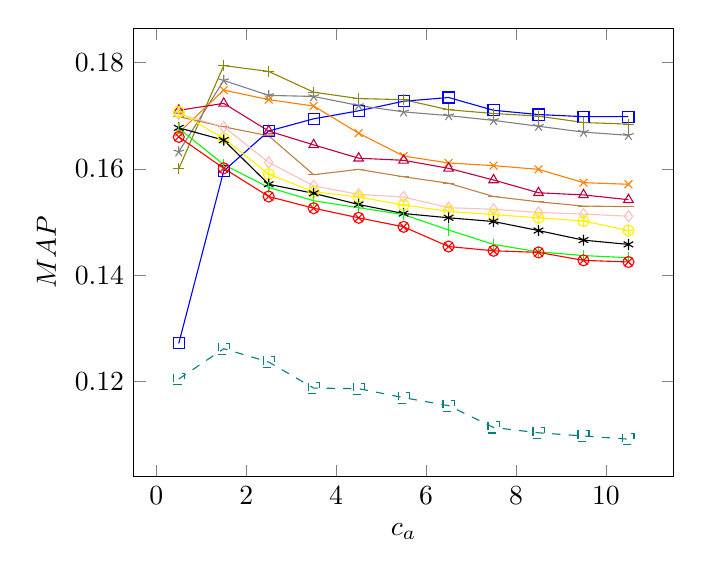
\begin{tikzpicture}
	\begin{axis}[
	 xlabel=$c_a$,
	ylabel=$MAP$,
	% y label style={rotate=-90},
	]

%%%%%%%%%%%%%%%%%%%%
%%% x=cv y=ca, from 5 to 50, with step of 5
%%%%%%%%%%%%%%%%%%%%
%%\addplot[mark=square, style=solid, color=blue] coordinates
%%{ ( , ) ( , ) ( , ) ( , ) ( , ) ( , ) ( , ) ( , ) ( , ) ( , ) ( , ) };

%\addplot[mark=+, style=solid, color=olive] coordinates
%{ (0, 0.1171) (5, 0.1608) (10 , 0.1506) (15 , 0.1448) (20 , 0.14) (25 , 0.1398) (30 , 0.139) (35 , 0.1381) (40 , 0.1371) (45 , 0.1368) (50 , 0.1361) };

%\addplot[mark=star, style=solid, color=gray] coordinates
%{ (0, 0.1098) (5 , 0.1539) (10 , 0.1436) (15 , 0.1378) (20 , 0.137) (25 , 0.1364) (30 , 0.136) (35 , 0.1351) (40 , 0.1347) (45 , 0.1342) (50 , 0.1338) };

%\addplot[mark=x, style=solid, color=orange] coordinates
%{ (0, 0.1073) (5, 0.1511) (10 , 0.1385) (15 , 0.1357) (20 , 0.1342) (25 , 0.1334) (30 , 0.1326) (35 , 0.132) (40 , 0.1312) (45 , 0.1308) (50 , 0.1282) };

%\addplot[mark=triangle, style=solid, color=purple] coordinates
%{ (0, 0.104) (5, 0.1483) (10 , 0.1365) (15 , 0.1337) (20 , 0.1327) (25 , 0.1322) (30 , 0.1312) (35 , 0.1311) (40 , 0.13) (45 , 0.1278) (50 , 0.1279) };

%\addplot[mark=-, style=solid, color=brown] coordinates
%{ (0, 0.1031) (5, 0.1464) (10 , 0.1347) (15 , 0.1327) (20 , 0.1317) (25 , 0.1314) (30 , 0.1306) (35 , 0.1302) (40 , 0.1295) (45 , 0.1274) (50 , 0.1269) };

%\addplot[mark=diamond, style=solid, color=pink] coordinates
%{ (0, 0.1024) (5, 0.1442) (10, 0.134) (15, 0.1321) (20, 0.1311) (25, 0.1309) (30, 0.1304) (35, 0.1293) (40, 0.1271) (45, 0.1268) (50, 0.1256) };

%\addplot[mark=oplus, style=solid, color=yellow] coordinates
%{ (0, 0.1019) (5, 0.1431) (10, 0.1331) (15, 0.1316) (20, 0.131) (25, 0.1304) (30, 0.1296) (35, 0.129) (40, 0.1265) (45, 0.126) (50, 0.1256) };

%\addplot[mark=asterisk, style=solid, color=black] coordinates
%{ (0, 0.1002) (5, 0.1428) (10, 0.1326) (15, 0.1311) (20, 0.1301) (25, 0.1298) (30, 0.1288) (35, 0.1285) (40, 0.1261) (45, 0.1258) (50, 0.1252) };

%\addplot[mark=|, style=solid, color=green] coordinates
%{ (0, 0.0988) (5, 0.1418) (10, 0.1322) (15, 0.1303) (20, 0.1293) (25, 0.1293) (30, 0.1284) (35, 0.1262) (40, 0.1253) (45, 0.1251) (50, 0.1247) };

%\addplot[mark=otimes, style=solid, color=red] coordinates
%{ (0, 0.0956) (5, 0.1415) (10, 0.1319) (15, 0.1301) (20, 0.129) (25, 0.1287) (30, 0.1279) (35, 0.1254) (40, 0.1251) (45, 0.1249) (50, 0.1242) };

%%%%%%%%%%%%%%%%%%%%
%%% x=ca y=cv, from 0.5 to 10.5, with step of 1
%%%%%%%%%%%%%%%%%%%%
\addplot[mark=square, style=dashed, color=teal] coordinates
{ (0.5, 0.1205) (1.5, 0.1262) (2.5, 0.1237) (3.5, 0.1188) (4.5, 0.1187) (5.5, 0.117) (6.5, 0.1155) (7.5, 0.1114) (8.5, 0.1104) (9.5, 0.1098) (10.5, 0.1092) };

\addplot[mark=square, style=solid, color=blue] coordinates
{ (0.5, 0.1272) (1.5, 0.1596) (2.5, 0.1671) (3.5, 0.1694) (4.5, 0.1709) (5.5, 0.1727) (6.5, 0.1734) (7.5, 0.171) (8.5, 0.1702) (9.5, 0.1698) (10.5, 0.1698) };

\addplot[mark=+, style=solid, color=olive] coordinates
{ (0.5, 0.16) (1.5, 0.1794) (2.5, 0.1783) (3.5, 0.1744) (4.5, 0.1732) (5.5, 0.173) (6.5, 0.1711) (7.5, 0.1704) (8.5, 0.1699) (9.5, 0.1687) (10.5, 0.1684) };

\addplot[mark=star, style=solid, color=gray] coordinates
{ (0.5, 0.1632) (1.5, 0.1766) (2.5, 0.1738) (3.5, 0.1736) (4.5, 0.1719) (5.5, 0.1707) (6.5, 0.17) (7.5, 0.1691) (8.5, 0.168) (9.5, 0.1669) (10.5, 0.1663) };

\addplot[mark=x, style=solid, color=orange] coordinates
{ (0.5, 0.1668) (1.5, 0.1748) (2.5, 0.173) (3.5, 0.1718) (4.5, 0.1667) (5.5, 0.1624) (6.5, 0.1611) (7.5, 0.1606) (8.5, 0.1599) (9.5, 0.1574) (10.5, 0.1571) };

\addplot[mark=triangle, style=solid, color=purple] coordinates
{ (0.5, 0.171) (1.5, 0.1723) (2.5, 0.1671) (3.5, 0.1645) (4.5, 0.162) (5.5, 0.1616) (6.5, 0.1601) (7.5, 0.1579) (8.5, 0.1555) (9.5, 0.1551) (10.5, 0.1542) };

\addplot[mark=-, style=solid, color=brown] coordinates
{ (0.5, 0.1698) (1.5, 0.1679) (2.5, 0.1662) (3.5, 0.1589) (4.5, 0.1599) (5.5, 0.1585) (6.5, 0.1573) (7.5, 0.1548) (8.5, 0.1538) (9.5, 0.153) (10.5, 0.1529) };

\addplot[mark=diamond, style=solid, color=pink] coordinates
{ (0.5, 0.1703) (1.5, 0.1679) (2.5, 0.1612) (3.5, 0.1568) (4.5, 0.1552) (5.5, 0.1547) (6.5, 0.1527) (7.5, 0.1524) (8.5, 0.1518) (9.5, 0.1515) (10.5, 0.1511) };

\addplot[mark=oplus, style=solid, color=yellow] coordinates
{ (0.5, 0.1707) (1.5, 0.1657) (2.5, 0.159) (3.5, 0.1557) (4.5, 0.1547) (5.5, 0.1532) (6.5, 0.152) (7.5, 0.1514) (8.5, 0.1508) (9.5, 0.1502) (10.5, 0.1484) };

\addplot[mark=asterisk, style=solid, color=black] coordinates
{ (0.5, 0.1677) (1.5, 0.1654) (2.5, 0.1571) (3.5, 0.1554) (4.5, 0.1533) (5.5, 0.1516) (6.5, 0.1508) (7.5, 0.1501) (8.5, 0.1484) (9.5, 0.1466) (10.5, 0.1458) };

\addplot[mark=|, style=solid, color=green] coordinates
{ (0.5, 0.1676) (1.5, 0.1608) (2.5, 0.1565) (3.5, 0.154) (4.5, 0.1527) (5.5, 0.1514) (6.5, 0.1485) (7.5, 0.1458) (8.5, 0.1444) (9.5, 0.1437) (10.5, 0.1433) };

\addplot[mark=otimes, style=solid, color=red] coordinates
{ (0.5, 0.166) (1.5, 0.1601) (2.5, 0.1548) (3.5, 0.1526) (4.5, 0.1508) (5.5, 0.1491) (6.5, 0.1454) (7.5, 0.1446) (8.5, 0.1443) (9.5, 0.1428) (10.5, 0.1425) };

\end{axis}
\end{tikzpicture}}

	\centering
	\caption{SS11}
\end{subfigure}


\subsection{Comparison between MF and Field-Based Models}
\label{sec:mf-field-cmp}

In this section, we evaluate and compare the performance of BM25 and PL2 ranking model against their MF extensions, BM25MF and PL2F respectively, and show the superiority of the MF model. TF-IDF is used as baseline.

\begin{description}
  \item[TF-IDF] is a logarithmic function of the term frequency and defines the Equation (\ref{eq:tfidf-score}) as 
  $
  tfn=log(f_{t,e})+1
  $,
  where $f_{t,e}$ is the number of occurrences of the term $t$ in the entity $e$.
  \item[BM25~\cite{robertson:1994:sigir}] considers the document as a simple bag of words. It is a function of the term frequency derived from a two-Poisson model and using an entity-length normalization. The entity length is computed as the sum of the \emph{attribute length} defined in the Section~\ref{sec:ranking-wod}. It defines the Equation (\ref{eq:tfidf-score}) as 
  $
  tfn=\frac{f_{t,e}\times(k_1+1)}{f_{t,e}+k_1\times \left(1+b\times\left(\frac{l_e}{l_{avg}}-1\right)\right)}
  $,
where $l_e$ is the \emph{entity length} of the entity $e$, $l_{avg}$ is the average of the \emph{entity length} in the collection and $b$ is a normalization parameter.
  \item[BM25F] is defined in Equation (\ref{eq:tfidf-score}). It considers documents as composed of fields, each field being a bag of words.
  \item[PL2~\cite{amati:2002:acm}] considers the document as a simple bag of words. It is a model derived from the DFR framework, with the Equation (\ref{eq:pl2f}) formulated as 
  $
  tfn=f_{t,e}\times log_2\left(1+c\times\frac{l_{avg}}{l_e}\right)
  $,
  where $c$ is a normalization parameter.
  \item[PL2F] is defined in Equation (\ref{eq:dfr-score}). It considers a document as a set of fields, each field being a bag of words.
\end{description}

\subsubsection{Comparison}

The Table~\ref{tab:norm-param} reports the values of the normalization parameters of each ranking function found through a constrained particle swarm optimization~\cite{xiaohui:2002:sci} on each dataset. Using such parameters, we report in Table~\ref{tab:final-results} the performance of the ranking functions on the three datasets. The $p$-Value is computed with the two-tailed Wilcoxon matched-pairs signed-ranks test~\cite{sheskin:2003:CRC,buttcher:2010:IRI:1869919}, where a statistically significant difference at level $0.10$ is marked with one star $*$ and at level $0.05$ with two stars $**$. BM25MF and PL2MF are used as a baseline in this test. $\Delta\%$ indicates the difference in percentage between the two MAP values compared in that test.
We note that for field-based ranking models and their MF extensions, the attribute label is considered as a value node, in order to be a source of potential relevant terms.

TF-IDF provides a clear-cut discrepancy between INEX09 and the datasets based on BTC, i.e., SS10 and SS11, the reason being it is not suited to heterogeneous datasets.
On SS10, BM25MF (resp., PL2MF) does not report a significant difference with BM25 (resp., PL2). On INEX09 and SS11, the MF extensions provide an increase of at least $10\%$ in retrieval performance compared to BM25 and PL2. On SS10 and SS11, the MF extensions provide better retrieval performance with a significant difference than the field-based ranking functions with an increase of $15\%$ at the minimum. On INEX09, BM25MF provides slightly better results than BM25F. Overall, the experiments show that the MF model improves significantly the ranking effectiveness.

\begin{table}
	\centering
	\ra{0.5}
	\begin{subfigure}{\textwidth}
		\centering
		\resizebox{\textwidth}{!}{
		\begin{tabular}{lc@{\hs}llrcllrc@{\hs}llrcllrc@{\hs}llrcllr}
			\toprule
			     & \phantom{a} & \multicolumn{7}{c}{INEX09}
			     & \phantom{a} & \multicolumn{7}{c}{SS10}
			     & \phantom{a} & \multicolumn{7}{c}{SS11} \\
			     \cmidrule{3-9} \cmidrule{11-17} \cmidrule{19-25}
			BM25MF & \phantom{a} & $b_a$ & $=$ & $0.00$ & \phantom{a} & $b_v$ & $=$ & $0.75$
			       & \phantom{a} & $b_a$ & $=$ & $0.58$ & \phantom{a} & $b_v$ & $=$ & $0.75$
			       & \phantom{a} & $b_a$ & $=$ & $0.58$ & \phantom{a} & $b_v$ & $=$ & $0.75$ \\
			BM25 & \phantom{a} & $b$ & $=$ & $0.20$ & \multicolumn{4}{c}{\phantom{a}}
			     & \phantom{a} & $b$ & $=$ & $0.20$ & \multicolumn{4}{c}{\phantom{a}}
			     & \phantom{a} & $b$ & $=$ & $0.20$ & \multicolumn{4}{c}{\phantom{a}} \\
			BM25F & \phantom{a} & $b_a$ & $=$ & $0.82$ & \multicolumn{4}{c}{\phantom{a}}
			      & \phantom{a} & $b_a$ & $=$ & $0.82$ & \multicolumn{4}{c}{\phantom{a}}
			      & \phantom{a} & $b_a$ & $=$ & $0.82$ & \multicolumn{4}{c}{\phantom{a}} \\
			\midrule
			PL2MF & \phantom{a} & $c_a$ & $=$ & $9.19$ & \phantom{a} & $c_v$ & $=$ & $0.76$
			      & \phantom{a} & $c_a$ & $=$ & $1.52$ & \phantom{a} & $c_v$ & $=$ & $1.03$
			      & \phantom{a} & $c_a$ & $=$ & $1.79$ & \phantom{a} & $c_v$ & $=$ & $1.88$ \\
			PL2 & \phantom{a} & $c$ & $=$ & $17.01$ & \multicolumn{4}{c}{\phantom{a}}
			    & \phantom{a} & $c$ & $=$ & $10.09$ & \multicolumn{4}{c}{\phantom{a}}
			    & \phantom{a} & $c$ & $=$ & $10.09$ & \multicolumn{4}{c}{\phantom{a}} \\
			PL2F & \phantom{a} & $c_a$ & $=$ & $1.87$ & \multicolumn{4}{c}{\phantom{a}}
			      & \phantom{a} & $c_a$ & $=$ & $0.51$ & \multicolumn{4}{c}{\phantom{a}}
			      & \phantom{a} & $c_a$ & $=$ & $1.51$ & \multicolumn{4}{c}{\phantom{a}} \\
			\bottomrule
		\end{tabular}}
		\caption{Normalization parameters values, found through a constrained particle swarm optimization.}
		\label{tab:norm-param}
	\end{subfigure}
	\qquad%
	\begin{subfigure}{\textwidth}
		\centering
		\resizebox{\textwidth}{!}{
		\begin{tabular}{lc@{\hs}rrccc@{\hs}rrccc@{\hs}rrcc}
			\toprule
			     & \phantom{a} & \multicolumn{4}{c}{INEX09}
			     & \phantom{a} & \multicolumn{4}{c}{SS10}
			     & \phantom{a} & \multicolumn{4}{c}{SS11} \\
			     & \phantom{a} & MAP & P@10 & $p$-Value & $\Delta\%$
			     & \phantom{a} & MAP & P@10 & $p$-Value & $\Delta\%$
			     & \phantom{a} & MAP & P@10 & $p$-Value & $\Delta\%$ \\
			\cmidrule{3-6} \cmidrule{8-11} \cmidrule{13-16}
			BM25MF & \phantom{a} & 0.1593 & 0.3982 & - & -
			       & \phantom{a} & 0.1303 & 0.3783 & - & -
			       & \phantom{a} & 0.1811 & 0.1880 & - & - \\
			TF-IDF & \phantom{a} & 0.1246 & 0.3109 & $3.2e^{-04**}$ & $-21.78$
			       & \phantom{a} & 0.0581 & 0.2304 & $2.1e^{-10**}$ & $-55.41$
			       & \phantom{a} & 0.0655 & 0.1040 & $1.4e^{-06**}$ & $-176.49$ \\
			BM25 & \phantom{a} & 0.1330 & 0.3309 & $8.4e^{-05**}$ & $-16.51$
			     & \phantom{a} & 0.1350 & 0.4000 & $3.7e^{-01}$ & -
			     & \phantom{a} &0.1625 & 0.1920 & $1.4e^{-01*}$ & $-11.45$ \\
			BM25F & \phantom{a} & 0.1489 & 0.3764 & $5.7e^{-03**}$ & $-6.53$
			      & \phantom{a} & 0.1100 & 0.3283 & $3.0e^{-05**}$ & $-15.58$
			      & \phantom{a} & 0.1401 & 0.1680 & $1.1e^{-04**}$ & $-29.26$ \\
			\midrule
			PL2MF & \phantom{a} & 0.1525 & 0.3800 & - & -
			      & \phantom{a} & 0.1232 & 0.3707 & - & -
			      & \phantom{a} & 0.1797 & 0.1880 & - & - \\
			TF-IDF & \phantom{a} & 0.1246 & 0.3109 & $5.4e^{-03**}$ & $-18.30$
			       & \phantom{a} & 0.0581 & 0.2304 & $5.4e^{-10**}$ & $-52.84$
			       & \phantom{a} & 0.0655 & 0.1040 & $6.9e^{-07**}$ & $-174.35$ \\
			PL2 & \phantom{a} & 0.1331 & 0.3218 & $6.0e^{-03**}$ & $-12.72$
			    & \phantom{a} & 0.1289 & 0.3946 & $4.1e^{-01}$ & -
			    & \phantom{a} & 0.1614 & 0.2000 & $3.3e^{-01*}$ & $-11.34$ \\
			PL2F & \phantom{a} & 0.1514 & 0.3473 & $7.7e^{-01}$ & -
			      & \phantom{a} & 0.1023 & 0.3163 & $2.4e^{-04**}$ & $-16.96$
			      & \phantom{a} & 0.1264 & 0.1560 & $4.5e^{-05**}$ & $-42.17$ \\
			\bottomrule
		\end{tabular}}
			\caption{Mean Average Precision (MAP) and the Precision at 10 (P@10) scores of PL2MF and BM25MF and the other state-of-the-art candidates; a $p$-Value is computed using the two-tailed Wilcoxon matched-pairs signed-ranks test, where one star $*$ marks statistically significant difference at level $0.10$, and two stars $**$ at level $0.05$, with BM25MF (resp., PL2MF) used as a baseline; $\Delta\%$ indicates the difference in percentage between the two MAP values compared in that test.}
			\label{tab:final-results}
	\end{subfigure}
	\caption{Comparison of state-of-the-art candidates against the MF generalizations.}
\end{table}


\subsection{Effectiveness of the Weights}
\label{sec:weights-effectiveness}

In this section, we discuss the impact of discarding the attribute label as a source of possible relevant terms on the ranking performance. Then we evaluate the weights from Section~\ref{sec:weights} developed for the MF model.
The Table~\ref{tab:mf-effect} reports the MAP scores of BM25MF and PL2MF combined with each weight individually and using the normalization parameters values from the Table~\ref{tab:norm-param}. Apart from the row ``Without Attribute Label'', all runs consider the attribute label as an additional value as in the previous experiments.

\subsubsection{\emph{The Impact of Attribute Label}}
\label{sec:with-att}

In this section, we investigate the consequence of not considering the attribute label as a source of relevant terms.
The Table~\ref{tab:mf-effect} reports under the \emph{BM25MF} and \emph{PL2MF} methods the results of considering or not the attribute label as an additional value.
We can see that removing the attribute label (\emph{Without Attribute Label} row) lowers the performance of the ranking with a statistical significance on INEX09 with BM25MF and PL2MF, and on SS11 with PL2MF only. This shows that the attribute labels can be a source of possible relevant terms.

\subsubsection{\emph{The Query Coverage Weight}}
\label{sec:qc-weight-effect}

In order to evaluate the benefit of the QC weight, we first analyse its effect separately when applied as an entity, an attribute or a value-specific weight. Then we study the consequence of applying it on all nodes at the same time (\emph{All} row). The Table~\ref{tab:mf-effect} reports the results under the \emph{BM25MF + QC} and \emph{PL2MF + QC} methods. QC improves the retrieval performance when applied on the attribute node, with a statistical significance on SS10 and SS11.

\subsubsection{\emph{The Value Coverage Weight}}
\label{sec:vc-weight-effect}

The evaluation of the VC weight investigates its efficiency with and without the function (\ref{eq:vc-norm}). The results are reported in Table~\ref{tab:mf-effect} under the \emph{BM25MF + VC} and \emph{PL2MF + VC} methods. We provide for each dataset the best performing $B$ and $\alpha$ parameters. We can observe that VC with the function (\ref{eq:vc-norm}) improves slightly the retrieval performance on SS10 and SS11. The reason is that, without this function, VC assigns a low weight to long values even if they have occurrences of all query terms.

\subsubsection{\emph{The Attribute and Entity Labels Weights}}
\label{sec:ael-weight-effect}

We evaluate the AEL weights first by considering the Attribute and the Entity Label weights separately, then both at the same time. The Table~\ref{tab:mf-effect} reports the results of applying such query-independent weights under the \emph{BM25MF + AEL} and \emph{PL2MF + AEL} methods.
We note that the Attribute Label weight gives significant benefits to the ranking in SS10 and SS11, while it decreases the ranking performance in INEX09. This indicates that carefully defined weights for important and non-important attributes can contribute significantly to the effectiveness of the approach. We note also that the same can be seen with the Entity Label weight applied alone. The reason is similar to the Attribute Label weight.
Except in INEX09, using both weights at the same time increases the performance of MF ranking functions noticeably.

\subsubsection{\emph{The Combination of Weights}}
\label{sec:combi-weight-effect}

In this section, we investigate the retrieval performance when all four weights are used together. We report the results in Table~\ref{tab:mf-effect} under the methods  \emph{BM25MF + AC + VC + AEL} and \emph{PL2MF + AC + VC + AEL}, with the weights configuration
\begin{inparaenum}[(1)]
    \item QC applied on the attribute node;
    \item VC with dataset-specific $B$ and $\alpha$ parameters; and
    \item AEL weights.
\end{inparaenum}
The weights applied on a same node are combined by the multiplication of each weight value on that node, i.e., either $b_a$ (resp., $c_a$) or $b_v$ (resp., $c_v$) weight values.
The attribute label being considered as a value, and the entity label being an additional attribute, we apply also the QC weight on those two labels in this experiment.
On INEX09 their combination decreases slightly the performance for PL2MF. On SS10 and SS11, although the QC and VC weights applied separately do not improve the effectiveness of the MF ranking functions by much, their combination with AEL increases the retrieval performance by at least $30\%$ on SS10 and SS11.

\begin{table*}
\centering
\ra{0.5}
\resizebox{\textwidth}{!}{%
\begin{tabular}{cc@{\hs}rrccc@{\hs}rrccc@{\hs}rrcc}
\toprule
Method & \phantom{a} & \multicolumn{4}{c}{INEX09}
                     & \phantom{a} & \multicolumn{4}{c}{SS10}
                     & \phantom{a} & \multicolumn{4}{c}{SS11} \\
 & \phantom{a} & MAP & P@10 & $p$-Value & $\Delta\%$
               & \phantom{a} & MAP & P@10 & $p$-Value & $\Delta\%$
               & \phantom{a} & MAP & P@10 & $p$-Value & $\Delta\%$ \\
\cmidrule{3-6} \cmidrule{8-11} \cmidrule{13-16}
\emph{\textbf{BM25MF}} & \multicolumn{15}{c}{\phantom{a}} \\
{\raggedright With Attribute Label} & \phantom{a} & 0.1593 & 0.3982 & - & -
                                    & \phantom{a} & 0.1303 & 0.3783 & - & -
                                    & \phantom{a} & 0.1811 & 0.1880 & - & - \\
{\raggedright Without Attribute Label} & \phantom{a} & 0.1484 & 0.3800 & $6.9e^{-04**}$ & $-6.84$
                                       & \phantom{a} & 0.1241 & 0.3783 & $4.5e-01$ & -
                                       & \phantom{a} & 0.1763 & 0.1940 & $8.6e-01$ & - \\
\\
\emph{\textbf{BM25MF + QC}} & \multicolumn{15}{c}{\phantom{a}} \\
{\raggedright Value} & \phantom{a} & 0.1482 & 0.3545 & $2.0e^{-01*}$ & $-6.97$
                     & \phantom{a} & 0.1325 & 0.3793 & $8.2e^{-01}$ & -
                     & \phantom{a} & 0.1841 & 0.2020 & $1.6e^{-01*}$ & $+1.66$ \\
% & Value - No IDF & \phantom{a} & 0.1449 & 22 & 32 & 1 %&  %&
%                  & \phantom{a} & 0.1330 & 30 & 26 & 36 %& 1.3108 %& 0.2667
%                  & \phantom{a} & 0.1835 & 19 & 17 & 14 %& 1.7108 %& 0.3473
%                  \\
{\raggedright Attribute} & \phantom{a} & 0.1624 & 0.3818 & $8.8e^{-01}$ & -
                         & \phantom{a} & 0.1339 & 0.3815 & $3.5e^{-01*}$ & $+2.76$
                         & \phantom{a} & 0.1841 & 0.2060 & $5.3e^{-02*}$ & $+1.66$ \\
% & Attribute - No IDF & \phantom{a} & 0.1589 & 22 & 32 & 1 %&  %&
%                      & \phantom{a} & 0.1362 & 30 & 20 & 42 %& 1.9128 %& 0.2674
%                      & \phantom{a} & 0.1840 & 22 & 13 & 15 %& 1.9298 %& 0.3458
%                      \\
{\raggedright Entity} & \phantom{a} & 0.1514 & 0.3782 & $4.0e^{-02*}$ & $-4.96$
                      & \phantom{a} & 0.1236 & 0.3728 & $2.8e^{-02**}$ & $-5.14$
                      & \phantom{a} & 0.1744 & 0.188 & $4.7e^{-01}$ & - \\
% & Entity - No IDF & \phantom{a} & \underline{0.1449} & 16 & 38 & 1 %&  % &
%                   & \phantom{a} & 0.1265 & 4 & 11 & 77 %& 1.8354 % & 0.2448
%                   & \phantom{a} & 0.1743 & 10 & 18 & 22 %& 1.8584 % & 0.3386
%                   \\
{\raggedright All} & \phantom{a} & 0.1506 & 0.3545 & $1.5e^{-01*}$ & $-5.46$
                   & \phantom{a} & 0.1263 & 0.3717 & $3.1e^{-01*}$ & $-3.07$
                   & \phantom{a} & 0.1810 & 0.2080 & $7.1e^{-01}$ & - \\
% & All - No IDF & \phantom{a} & \underline{0.1392} & 21 & 34 & 0 %&  % &
%                & \phantom{a} & 0.1263 & 30 & 35 & 27 %& 1.7154 % & 0.2505
%                & \phantom{a} & 0.1744 & 15 & 24 & 11 %& 1.7458 % & 0.3304
%                \\
\\
\emph{\textbf{BM25MF + LC}} & \multicolumn{15}{c}{\phantom{a}} \\
\multirow{2}{*}{{\raggedright With Control Function (\ref{chap6:ranking:eq:lc-norm})}} & \phantom{a} & 0.1606 & 0.3964 & $2.8e^{-01*}$ & $+0.82$
                                                                 & \phantom{a} & 0.1321 & 0.3761 & $3.7e^{-01}$ & -
                                                                 & \phantom{a} & 0.1802 & 0.1920 & $5.4e^{-01}$ & - \\
 & \phantom{a} & \multicolumn{4}{c}{$n=1,\;\alpha=0.7$}
   & \phantom{a} & \multicolumn{4}{c}{$n=2,\;\alpha=0.4$}
   & \phantom{a} & \multicolumn{4}{c}{$n=1,\;\alpha=0.9$} \\
{\raggedright Without Control Function (\ref{chap6:ranking:eq:lc-norm})} & \phantom{a} & 0.1293 & 0.3055 & $8.9e^{-04**}$ & $-18.83$
                                                   & \phantom{a} & 0.1260 & 0.3609 & $5.3e^{-01}$ & -
                                                   & \phantom{a} & 0.1296 & 0.1820 & $2.1e^{-03**}$ & $-39.74$ \\
\\
\emph{\textbf{BM25MF + AEL}} & \multicolumn{15}{c}{\phantom{a}} \\
{\raggedright Entity Label Weight} & \phantom{a} & 0.1574 & 0.3909 & $9.1e^{-02*}$ & $-1.19$
                                   & \phantom{a} & 0.1401 & 0.4011 & $7.8e^{-05**}$ & $+7.52$
                                   & \phantom{a} & 0.1937 & 0.2000 & $6.1e^{-03**}$ & $+6.96$ \\
{\raggedright Attribute Label Weight} & \phantom{a} & 0.1604 & 0.3982 & $4.3e^{-01}$ & -
                                      & \phantom{a} & 0.1504 & 0.4228 & $2.6e^{-06**}$ & $+15.43$
                                      & \phantom{a} & 0.2173 & 0.2360 & $6.8e^{-06**}$ & $+19.99$ \\
{\raggedright Both} & \phantom{a} & 0.1593 & 0.3982 & $4.4e^{-01}$ & -
                    & \phantom{a} & 0.1584 & 0.4391 & $2.0e^{-07**}$ & $+21.57$
                    & \phantom{a} & 0.2274 & 0.2420 & $2.7e^{-05**}$ & $+25.57$ \\
\\
\emph{\textbf{BM25MF + QC + LC + AEL}} & \phantom{a} & 0.1589 &  & $5.9e^{-01}$ & -
                                       & \phantom{a} & 0.1720 & 0.4620 & $3.8e^{-06**}$ & $+32.00$
                                       & \phantom{a} & 0.2416 & 0.2560 & $1.1e^{-05**}$ & $+33.41$ \\
\midrule
\\[-0.2cm]

\emph{\textbf{PL2MF}} & \multicolumn{15}{c}{\phantom{a}} \\
{\raggedright With Attribute Label} & \phantom{a} & 0.1525 & 0.3800 & - & -
                                    & \phantom{a} & 0.1232 & 0.3685 & - & -
                                    & \phantom{a} & 0.1797 & 0.1880 & - & -
                        \\
{\raggedright Without Attribute Label} & \phantom{a} & 0.1401 & 0.3618 & $2.3e^{-04**}$ & $-8.13$
                                       & \phantom{a} & 0.1192 & 0.3674 & $5.3e^{-01}$ & -
                                       & \phantom{a} & 0.1680 & 0.1840 & $1.6e^{-01*}$ & $-6.51$
                           \\
\\
\emph{\textbf{PL2MF + QC}} & \multicolumn{15}{c}{\phantom{a}} \\
{\raggedright Value} & \phantom{a} & 0.1348 & 0.3382 & $1.0e^{-03**}$ & $-11.61$
                     & \phantom{a} & 0.1276 & 0.3750 & $2.8e^{-01*}$ & $+3.57$
                     & \phantom{a} & 0.1818 & 0.1980 & $1.6e^{-01*}$ & $+1.17$
         \\
% & Value - No IDF & \phantom{a} & \underline{0.1339} & 19 & 33 & 3 %&  %& 0.2892
%                  & \phantom{a} & \underline{0.1270} & 38 & 20 & 34 %& \underline{1.9616} %& 0.2530
%                  & \phantom{a} & \underline{0.1804} & 24 & 11 & 15 %& \underline{1.9606} %& 0.3477
%                  \\
{\raggedright Attribute} & \phantom{a} & 0.1569 & 0.3793 & $8.4e^{-01}$ & -
                         & \phantom{a} & 0.1299 & 0.3761 & $1.6e^{-01*}$ & $+5.44$
                         & \phantom{a} & 0.1815 & 0.1960 & $6.5e^{-02*}$ & $+1.00$
             \\
% & Attribute - No IDF & \phantom{a} & 0.1550 & 28 & 25 & 2 %& 0.9834 %& 0.3050
%                      & \phantom{a} & \underline{0.1270} & 32 & 17 & 43 %& \underline{1.9736} %& 0.2539
%                      & \phantom{a} & \underline{0.1796} & 23 & 12 & 15 %& \underline{1.9700} %& 0.3453
%                      \\
{\raggedright Entity} & \phantom{a} & 0.1499 & 0.3727 & $3.9e^{-01}$ & -
                      & \phantom{a} & 0.1168 & 0.3609 & $3.8e^{-02**}$ & $-5.19$
                      & \phantom{a} & 0.1655 & 0.1900 & $1.2e^{-01*}$ & $-7.90$
          \\
% & Entity - No IDF & \phantom{a} & 0.1431 & 24 & 30 & 1 %& 0.0892 %& 0.2884
%                   & \phantom{a} & 0.1175 & 5 & 9 & 78 %& 0.2584 %& 0.2400
%                   & \phantom{a} & 0.1630 & 8 & 20 & 22 %& 0.0174 %& 0.3278
%                   \\
{\raggedright All} & \phantom{a} & 0.1374 & 0.3309 & $1.5e^{-02**}$ & $-9.90$
                   & \phantom{a} & 0.1257 & 0.3728 & $6.4e^{-01}$ & -
                   & \phantom{a} & 0.1743 & 0.2020 & $9.4e^{-01}$ & $-3.01$
       \\
% & All - No IDF & \phantom{a} & \underline{0.1296} & 17 & 38 & 0 %& 0.0032 %& 0.2790
%                & \phantom{a} & 0.1211 & 32 & 31 & 29 %& 0.5754 %& 0.2426
%                & \phantom{a} & 0.1680 & 17 & 21 & 12 %& 0.4592 %& 0.3270
%                \\
\\
\emph{\textbf{PL2MF + LC}} & \multicolumn{15}{c}{\phantom{a}} \\
\multirow{2}{*}{{\raggedright With Function (\ref{chap6:ranking:eq:lc-norm})}} & \phantom{a} & 0.1494 & 0.3673 & $1.5e^{-02**}$ & $-2.03$
                                                & \phantom{a} & 0.1253 & 0.3663 & $2.4e^{-01*}$ & $+1.70$
                                                & \phantom{a} & 0.1802 & 0.1900 & $1.4e^{-01*}$ & $+0.29$ \\%[-0.05in]
 & \phantom{a} & \multicolumn{4}{c}{$n=1,\;\alpha=0.7$}
   & \phantom{a} & \multicolumn{4}{c}{$n=2,\;\alpha=0.4$}
   & \phantom{a} & \multicolumn{4}{c}{$n=1,\;\alpha=0.9$} \\
{\raggedright Without Function (\ref{chap6:ranking:eq:lc-norm})} & \phantom{a} & 0.1182 & 0.2909 & $5.4e^{-07**}$ & $-21.84$
                                                   & \phantom{a} & 0.1179 & 0.3391 & $3.8e^{-01}$ & -
                                                   & \phantom{a} & 0.1466 & 0.1900 & $7.3e^{-03**}$ & $-18.42$
                                       \\
\\
\emph{\textbf{PL2MF + AEL}} & \multicolumn{15}{c}{\phantom{a}} \\
{\raggedright Entity Label Weight} & \phantom{a} & 0.1523 & 0.3800 & $2.5e^{-01*}$ & $-0.13$
                                   & \phantom{a} & 0.1305 & 0.3848 & $6.4e^{-06**}$ & $+5.93$
                                   & \phantom{a} & 0.1824 & 0.1920 & $4.4e^{-02*}$ & $+1.50$
                       \\
{\raggedright Attribute Label Weight} & \phantom{a} & 0.1521 & 0.3673 & $1.9e^{-02**}$ & $-0.26$
                                      & \phantom{a} & 0.1471 & 0.4163 & $3.7e^{-07**}$ & $+19.40$
                                      & \phantom{a} & 0.2150 & 0.2320 & $4.0e^{-05**}$ & $+19.64$
                          \\
{\raggedright Both} & \phantom{a} & 0.1516 & 0.3709 & $1.2e^{-02**}$ & $-0.59$
                    & \phantom{a} & 0.1542 & 0.4337 & $3.4e^{-09**}$ & $+25.16$
                    & \phantom{a} & 0.2187 & 0.2380 & $1.2e^{-05**}$ & $+21.70$
        \\
\\
\emph{\textbf{PL2MF + QC + LC + AEL}} & \phantom{a} & 0.1492 & 0.3582 & $1.5e^{-01*}$ & $-2.16$
                                      & \phantom{a} & 0.1717 & 0.4620 & $2.0e^{-08**}$ & $+39.36$
                                      & \phantom{a} & 0.2360 & 0.2520 & $2.5e^{-05**}$ & $+31.33$ \\
\bottomrule
\end{tabular}}
\caption{Evaluation of the weights effectiveness on PL2MF and BM25MF.% effectiveness. Mean Average Precision (MAP) scores of each BM25MF and PL2MF with each weight individually; using the two-tailed Wilcoxon matched-pairs signed-ranks test, a $p$-Value with one star $*$ marks statistically significant difference at level $0.10$, and two stars $**$ at level $0.05$, with the baseline, i.e., BM25MF (respectively, PL2MF); $\Delta\%$ indicates the difference in percentage between the two MAP values.
}
\label{tab:mf-effect}
\end{table*}

